\documentclass[border=20pt, tikz]{standalone}
\usepackage{amsmath}
\usetikzlibrary{calc, arrows.meta}

% =========================================================
% GLOBAL SETTINGS
% Applies uniformly to all diagrams on all pages
% (Note: No blank lines allowed inside \tikzset)
% =========================================================
\tikzset{
    glass/.style={fill=cyan!20, draw=cyan!70!blue, thick, fill opacity=0.35, line join=round},
    glassfront/.style={fill=cyan!30, draw=cyan!80!blue, thick, fill opacity=0.6, line join=round},
    axis/.style={thick, -{Latex[length=3mm, width=2mm]}},
    common settings/.style={
        font=\sffamily\small,
        x={(0.9cm, -0.15cm)}, 
        y={(0cm, 1cm)}, 
        z={(-0.6cm, -0.5cm)}
    }
}

\begin{document}



% =========================================================
% PAGE 2: ORTHOGRAPHIC CUBOID
% =========================================================
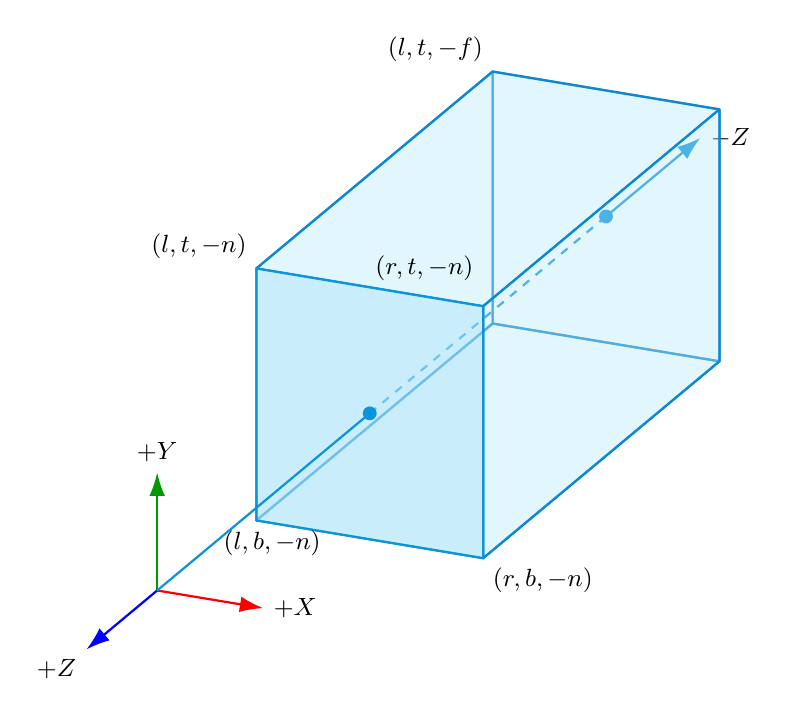
\begin{tikzpicture}[common settings]
    
    \def\n{4.5}  % Near plane distance
    \def\f{9.5}  % Far plane distance
    \def\s{1.6}  % Constant bounds for ortho (left/right/top/bottom)

    % Far Face (Background)
    \path[glass] (-\s,-\s,-\f) -- (\s,-\s,-\f) -- (\s,\s,-\f) -- (-\s,\s,-\f) -- cycle;
    
    % Left and Bottom Faces
    \path[glass] (-\s,-\s,-\f) -- (-\s,\s,-\f) -- (-\s,\s,-\n) -- (-\s,-\s,-\n) -- cycle; % Left
    \path[glass] (-\s,-\s,-\f) -- (\s,-\s,-\f) -- (\s,-\s,-\n) -- (-\s,-\s,-\n) -- cycle; % Bottom
    
    % Coordinate Axes at Origin
    \draw[axis, red] (0,0,0) -- (1.5,0,0) node[right, text=black] {$+X$};
    \draw[axis, green!60!black] (0,0,0) -- (0,1.5,0) node[above, text=black] {$+Y$};
    \draw[axis, blue] (0,0,0) -- (0,0,1.5) node[below left, text=black] {$+Z$};

    % Z-axis traversing the cuboid
    
    \draw[cyan!80!blue, thick, dashed] (0,0,-\n) -- (0,0,-\f); 
    \draw[axis, cyan!80!blue] (0,0,-\f) -- (0,0,-\f-2) node[right, text=black] {$-Z$}; 
    
    
    \fill[cyan!80!blue] (0,0,-\f) circle (2.5pt);

    % Top and Right Faces
    \path[glass] (-\s,\s,-\f) -- (\s,\s,-\f) -- (\s,\s,-\n) -- (-\s,\s,-\n) -- cycle; % Top
    \path[glass] (\s,-\s,-\f) -- (\s,\s,-\f) -- (\s,\s,-\n) -- (\s,-\s,-\n) -- cycle; % Right

    % Near Face (Foreground)
    \path[glassfront] (-\s,-\s,-\n) -- (\s,-\s,-\n) -- (\s,\s,-\n) -- (-\s,\s,-\n) -- cycle;

    % Intersection Dots
    \fill[cyan!80!blue] (0,0,-\n) circle (2.5pt);
    \draw[cyan!80!blue, thick] (0,0,0) -- (0,0,-\n); 

    % Math Labels
    \node[above left] at (-\s, \s, -\n) {$(l, t, -n)$};
    \node[above left] at (-\s, \s, -\f) {$(l, t, -f)$};
    \node[above left] at (\s, \s + 0.2, -\n) {$(r, t, -n)$};
    \node[below right] at (-\s - 0.6, -\s - 0.1 , -\n) {$(l, b, -n)$};
    \node[below right] at (\s, -\s, -\n) {$(r, b, -n)$};
    
\end{tikzpicture}


\end{document}